\documentclass{report}
\usepackage{graphicx}
\usepackage{enumitem}
\usepackage{multicol}
\usepackage[margin=2cm]{geometry}
\usepackage{hyperref}

\title{\Huge \textbf{Use Cases}\\ \huge Arfib}
\author{
    Henrique Romão \\ up202108067@up.pt
    \and
    Mariana Bessa \\ up202107946@up.pt
}

\setlength{\parindent}{0px}
\setlength{\parskip}{1em}

\begin{document}

\maketitle

\begin{abstract}
    E
\end{abstract}

\tableofcontents

\chapter{Requirements}
An app is being developed for atrial fibrilation monitoring.
This app is used by both patients monitoring this condition and respective doctors. 
This way, the app should allow for both patient and doctor separate interfaces.

A main part of this app is the ability to measure ECG signals, and display them in real-time while being measured.
A patient has to have the ability to make new measurements as well as consult old ones.
Each measurement should be analyzed, storing that information with the measurement result.

\textit{[Patient Symptoms]}

Patients can also track their medication in the app.
They should be able to log the medication that they need to take in each day, and see in which days they need to take which medications.
For each medication certain information needs to be available to see and edit, if needed, and patients can add new medication filling out the required information.
Patients should be able to see all medications in a simple view.

There is a blog inside the app, in which authorized personel can publish different posts.
There should be an interface in which patients can see the blog posts and read each one in a dedicated page.

\textit{[Doctor Interface]}


\newpage
\chapter{Use Case Diagram}

\section{Actors}
Considering the system requirements, it was possible to identify the actors represented in Figure \ref{fig:Actors}.

\subsection{Diagram}
\begin{figure}[ht]
    \centering
    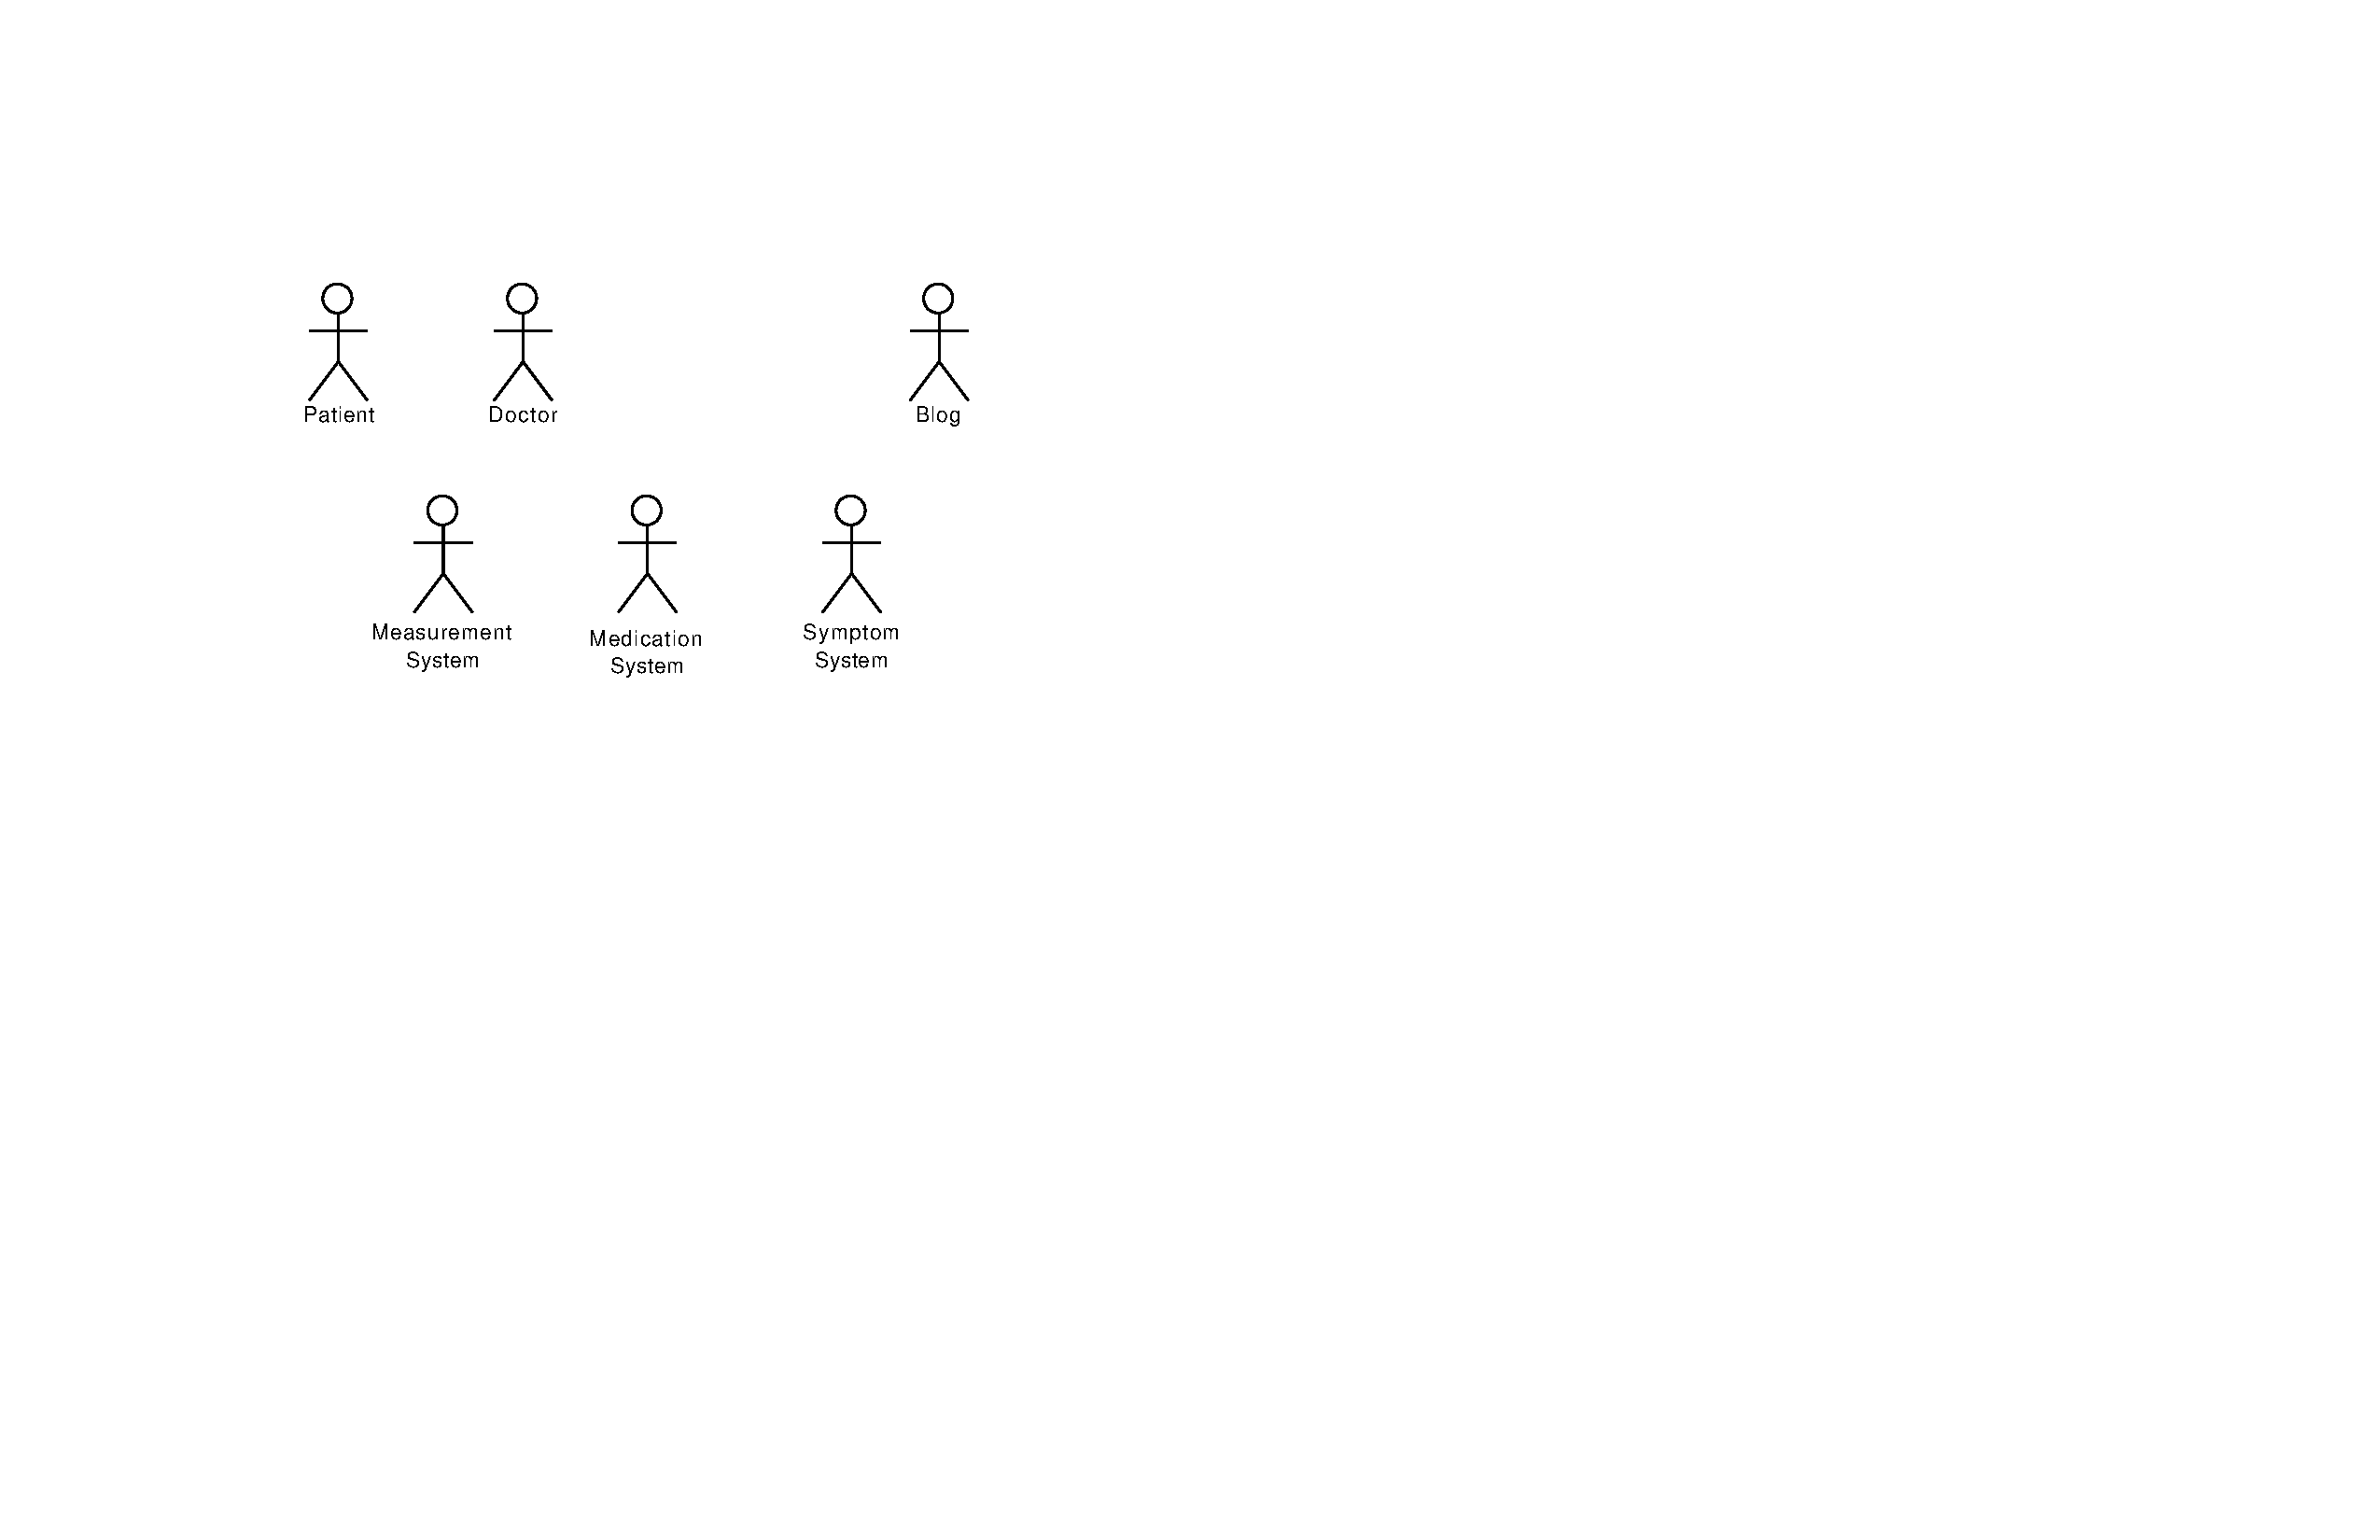
\includegraphics[width=0.5\linewidth]{Actors.pdf}
    \caption{Actors.}
    \label{fig:Actors}
\end{figure}

\subsection{Patient}
\subsection{Doctor}
\subsection{Measurement System}
\subsection{Medication System}
\subsection{Symptom System}
\subsection{Blog}

\clearpage
\section{Use Cases}
Considering the actors and system requirements, the following diagram represents the use cases for this system.

\begin{figure}[hb]
    \centering
    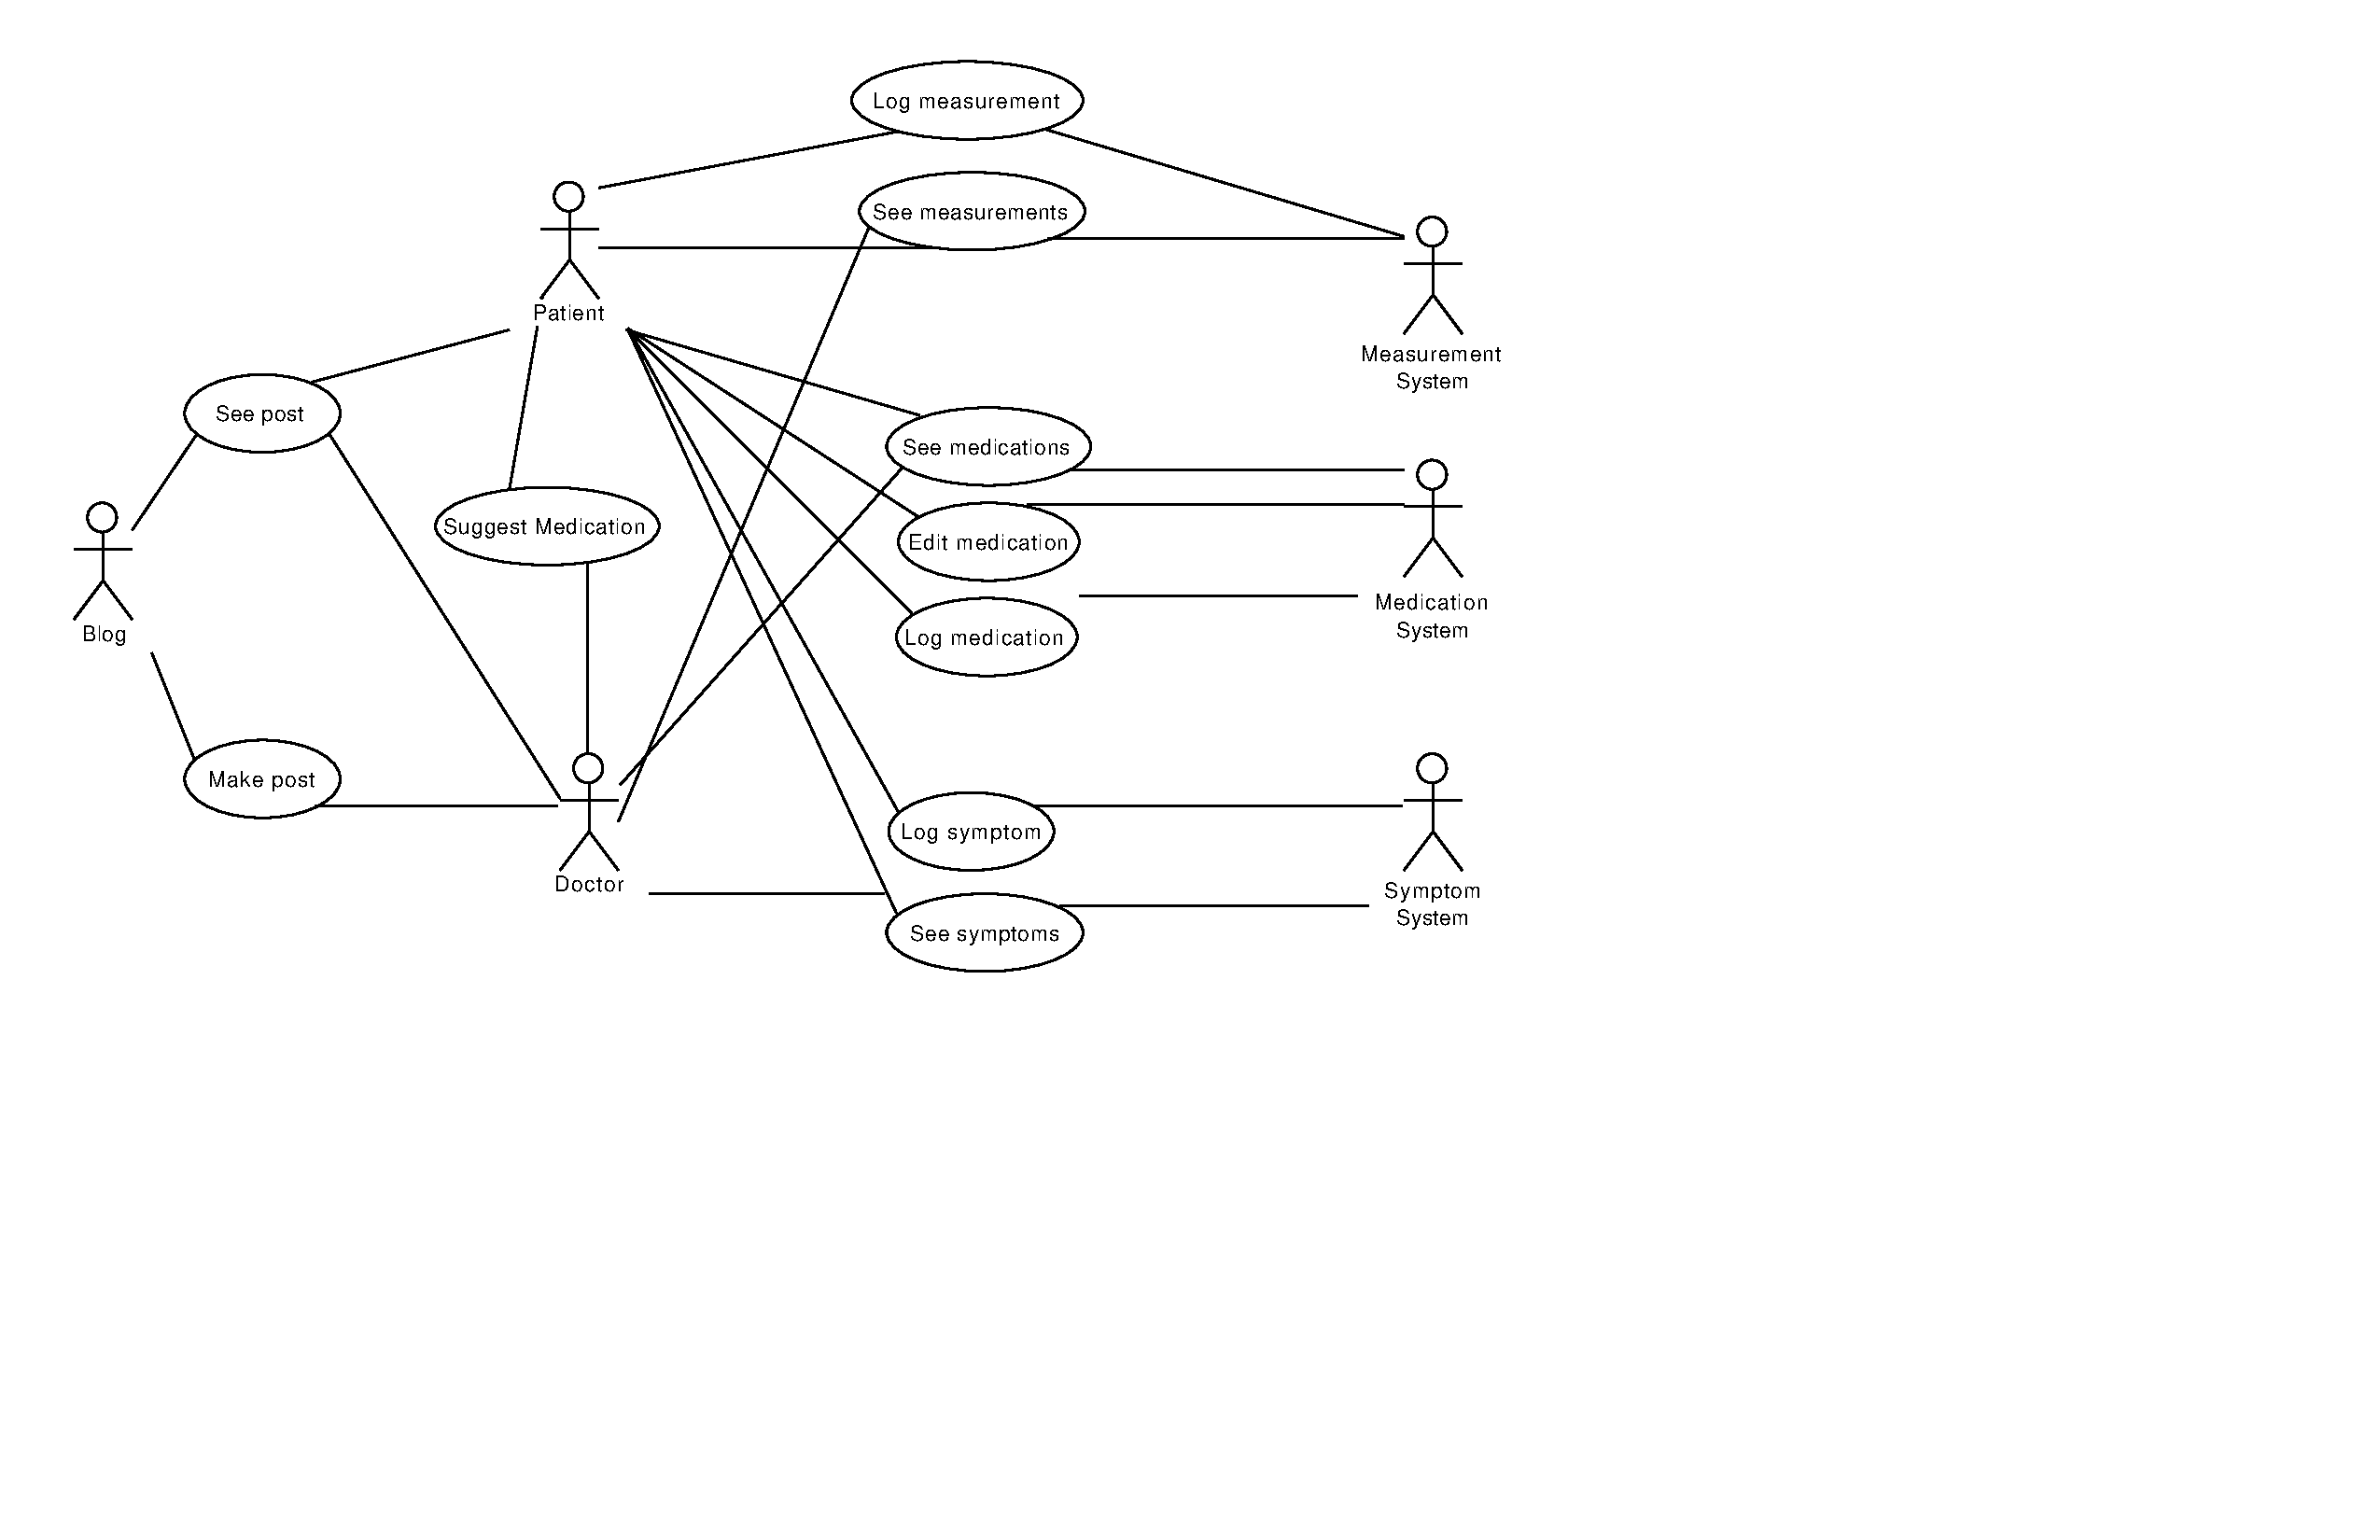
\includegraphics[width=\linewidth]{General Use Case Diagram.pdf}
    \caption{Use Case Diagram.}
    \label{fig:Use Case}
\end{figure}

\chapter{Use Case Description}
\vspace{-3em}
\section{Measurement}
\subsection{Log Measurement}
\vspace{-1em}
\paragraph{Brief Description}
This use case allows a patient to perform an ECG measurement using a device of their choosing. 
The patient must select a valid device, being abble to add new devices.
The measurement is shown in real time and can be stopped during the process.

\vspace{-1em}
\subsubsection{Flow of Events}
\begin{figure}[ht]
    \centering
    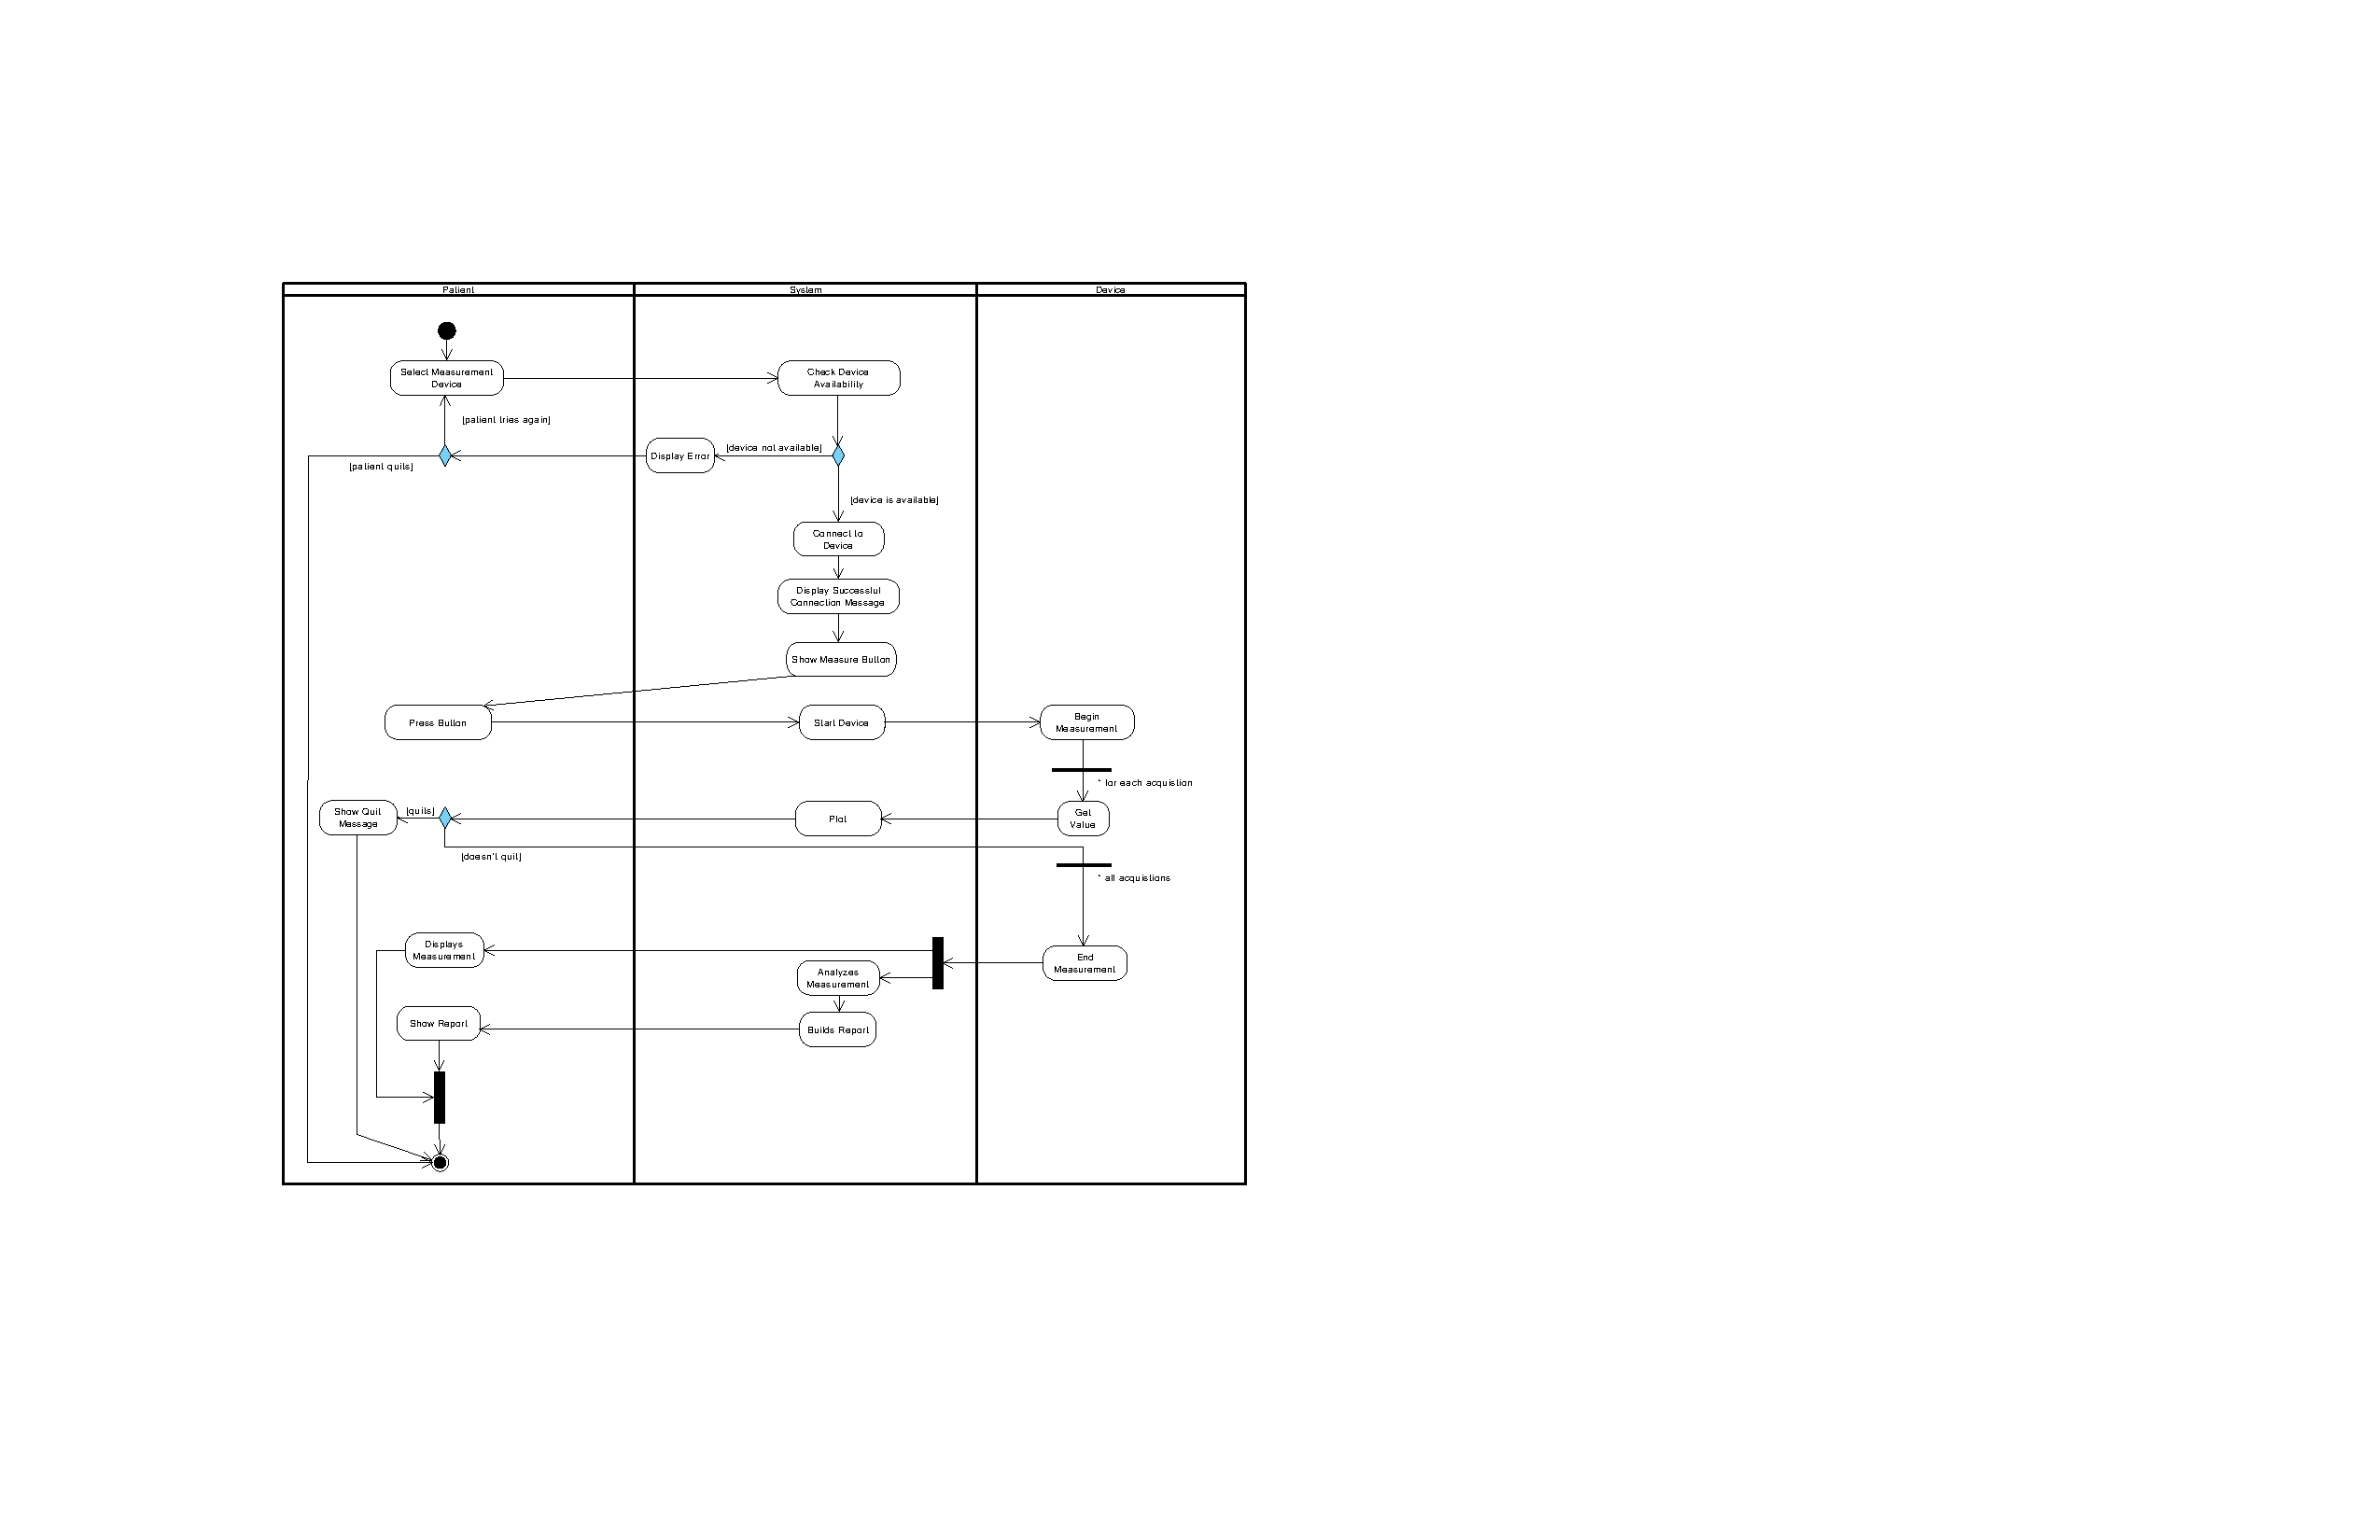
\includegraphics[width=0.7\linewidth]{Log Measurement.pdf}
    \caption{Log Measurement Activity Diagram.}
    \label{fig:Log Measure}
\end{figure}

\clearpage
\subsection{See Measurement}

\paragraph{Brief Description}
This use case allows a patient see its own previous measurements, or allows a doctor to see the previous measurements of their patients.
Both have access to a list of the measurments, allowing them to choose a specific one to see in more detail.

\begin{multicols}{2}
    \paragraph{Basic Flow}
    \begin{enumerate}
        \item Select patient's measurements page.
        \item Check access.
        \item Display previous measurements.
        \item Choose measurement of interest.
        \item Display full information about measurement of interest.
    \end{enumerate}
    \columnbreak
    
    \paragraph{Alternative Flows}
    \begin{enumerate}[label=A\arabic*.]
        \item Doctor or patient does not have access.
        \item Show error message.
        \item Quit.
        \item See measurement closed.
    \end{enumerate}
\end{multicols}

\vspace{1em}
\section{Medications}
\subsection{Log Medication}
\paragraph{Brief Description}
This use case allows a patient to affirme if they have taken their medication, and store that information.

\begin{multicols}{2}
    \paragraph{Basic Flow}
    \begin{enumerate}
        \item Select medication to log.
        \item Confirm medication has been taken.
        \item Change medication status.
    \end{enumerate}
    \columnbreak

    \paragraph{Alternative Flows}
    \begin{enumerate}[label=A\arabic*.]
        \item Select medication to remove log.
        \item Confirm mistake.
        \item Change status of the mistakenly logged medication.
    \end{enumerate}
\end{multicols}

\vspace{1em}
\subsection{See Medications}
\paragraph{Brief Description}
This use case allows a patient see its medications and respective logs, or allows a doctor to see the medications and logs of their patients.
Both have access to the medication's logs and to the medications' information.

\begin{multicols}{2}
    \paragraph{Basic Flow}
    \begin{enumerate}
        \item Select patient's medications page.
        \item Check access.
        \item Display medication logs.
        \item Choose medication of interest.
        \item Display information about medication of interest.
    \end{enumerate}
    \columnbreak

    \paragraph{Alternative Flows}
    \begin{enumerate}[label=A\arabic*.]
        \item Doctor or patient does not have access.
        \item Show error message.
        \item Quit.
        \item See medication closed.
    \end{enumerate}
\end{multicols}

\vspace{1em}
\subsection{Edit Medication}
\paragraph{Brief Description}
Allows the patient to change information regarding their medication, such as intake quantity, frequency and select an end date, from which the medication will not need to be taken.
Also, the use case allows adding new medications.

\begin{multicols}{2}
    \paragraph{Basic Flow}
    \begin{enumerate}
        \item Select medication.
        \item Enter edit mode.
        \item Choose parameter to change.
        \item Exit edit mode.
    \end{enumerate}
    \columnbreak

    \paragraph{Alternative Flows}
    \begin{enumerate}[label=A\arabic*.]
        \item Select new medication.
        \item Fill the required information.
        \item Add new medication.
    \end{enumerate}
\end{multicols}

\vspace{1em}
\subsection{Suggest Medication}
\paragraph{Brief Description}
This use case allows a doctor to suggest a new medication for a given patient.

\paragraph{Basic Flow}
\begin{enumerate}
    \item Select patient.
    \item Select medication.
    \item Fill the required information.
    \item Check information.
    \item Send to patient.
    \item Alert patient of suggestion.
\end{enumerate}
% [COMMENT][HENRIQUE] aqui não estou a ver nenhum alternative flow

\vspace{1em}
\section{Symptoms}
\subsection{Log Symptom}
\paragraph{Brief Description}
Text

\begin{multicols}{2}
    \paragraph{Basic Flow}
    \begin{enumerate}
        \item .
    \end{enumerate}
    \columnbreak

    \paragraph{Alternative Flows}
    \begin{enumerate}[label=A\arabic*.]
        \item .
    \end{enumerate}
\end{multicols}

\vspace{1em}
\subsection{See Symptoms}
\paragraph{Brief Description}
Text

\begin{multicols}{2}
    \paragraph{Basic Flow}
    \begin{enumerate}
        \item .
    \end{enumerate}
    \columnbreak

    \paragraph{Alternative Flows}
    \begin{enumerate}[label=A\arabic*.]
        \item .
    \end{enumerate}
\end{multicols}

\vspace{1em}
\section{Blog}
\subsection{See Post}
\paragraph{Brief Description}
Text

\begin{multicols}{2}
    \paragraph{Basic Flow}
    \begin{enumerate}
        \item .
    \end{enumerate}
    \columnbreak

    \paragraph{Alternative Flows}
    \begin{enumerate}[label=A\arabic*.]
        \item .
    \end{enumerate}
\end{multicols}

\vspace{1em}
\subsection{Publish Post}
\paragraph{Brief Description}
Text

\begin{multicols}{2}
    \paragraph{Basic Flow}
    \begin{enumerate}
        \item .
    \end{enumerate}
    \columnbreak

    \paragraph{Alternative Flows}
    \begin{enumerate}[label=A\arabic*.]
        \item .
    \end{enumerate}
\end{multicols}

\end{document}